\documentclass[a4paper,10pt]{article}
\usepackage[utf8]{inputenc}
\usepackage[a4paper,
            bindingoffset=0.2in,
            left=1in,
            right=1in,
            top=1in,
            bottom=1in,
            footskip=.25in]{geometry}

%###############################################################################

%\input{~/layout/global_layout}


%###############################################################################

% packages begin

\usepackage[
  backend=biber,
  sortcites=true,
  style=alphabetic,
  eprint=true,
  backref=true
]{biblatex}
\addbibresource{bibliographie.bib}
\usepackage[acronym]{glossaries}

\usepackage{euscript}[mathcal]
% e.g. \mathcal{A} for fancy letters in mathmode
\usepackage{amsmath,amssymb,amstext,amsthm}

\usepackage{mdframed}
\newmdtheoremenv[nobreak=true]{problem}{Problem}[subsection]
\newmdtheoremenv[nobreak=true]{claim}{Claim}[subsection]
\newtheorem{definition}{Definition}[subsection]
\newtheorem{lemma}{Lemma}[claim]
\newtheorem{plemma}{Lemma}[problem]

\usepackage{mathtools}
\DeclarePairedDelimiter\ceil{\lceil}{\rceil}
\DeclarePairedDelimiter\floor{\lfloor}{\rfloor}

\usepackage{enumerate}
\usepackage[pdftex]{graphicx}
\usepackage{subcaption}
% 'draft' für schnelleres rendern mitübergeben -> [pdftex, draft]
% dadruch wird nicht das bild mitgerendered, sondern nur ein kasten mit bildname -> schont ressourcen

\usepackage{hyperref}

\usepackage{tikz}
\usetikzlibrary{arrows,automata,matrix,positioning,shapes}

% for adding non-formatted text to include source-code
\usepackage{listings}
\lstset{language=Python,basicstyle=\footnotesize}
% z.B.:
% \lstinputlisting{source_filename.py}
% \lstinputlisting[lanugage=Python, firstline=37, lastline=45]{source_filename.py}
%
% oder
%
% \begin{lstlisting}[frame=single]
% CODE HERE
%\end{lstlisting}
\usepackage{algorithm}
\usepackage{algpseudocode}

\usepackage{wasysym}

\usepackage{titling}
\usepackage{titlesec}
\usepackage[nocheck]{fancyhdr}
\usepackage{lastpage}

\usepackage{kantlipsum}
\usepackage[colorinlistoftodos,prependcaption,textsize=tiny]{todonotes}

% packages end
%###############################################################################

\pretitle{% add some rules
  \begin{center}
    \LARGE\bfseries
} %, make the fonts bigger, make the title (only) bold
\posttitle{%
  \end{center}%
  %\vskip .75em plus .25em minus .25em% increase the vertical spacing a bit, make this particular glue stretchier
}
\predate{%
  \begin{center}
    \normalsize
}
\postdate{%
  \end{center}%
}

\titleformat*{\section}{\Large\bfseries}
\titleformat*{\subsection}{\large\bfseries}
\titleformat*{\subsubsection}{\normalsize\bfseries}

\titleformat*{\paragraph}{\Large\bfseries}
\titleformat*{\subparagraph}{\large\bfseries}

%###############################################################################

\pagestyle{fancy}
\fancyhf{}
% l=left, c=center, r=right; e=even_pagenumber, o=odd_pagenumber; h=header, f=footer
% example: [lh] -> left header, [lof,ref] -> fotter left when odd, right when even
%\fancyhf[lh]{}
%\fancyhf[ch]{}
%\fancyhf[rh]{}
%\fancyhf[lf]{}
\fancyhf[cf]{\footnotesize Page \thepage\ of \pageref*{LastPage}}
%\fancyhf[rf]{}
\renewcommand{\headrule}{} % removes horizontal header line

% Fotter options for first page

\fancypagestyle{firstpagestyle}{
  \renewcommand{\thedate}{\textmd{}} % removes horizontal header line
  \fancyhf{}
  \fancyhf[lh]{\ttfamily M.Sc. Computer Science\\KTH Royal Institute of Technology}
  \fancyhf[rh]{\ttfamily Period 4\\\today}
  \fancyfoot[C]{\footnotesize Page \thepage\ of \pageref*{LastPage}}
  \renewcommand{\headrule}{} % removes horizontal header line
}
%###############################################################################

\newcommand\extrafootertext[1]{%
    \bgroup
    \renewcommand\thefootnote{\fnsymbol{footnote}}%
    \renewcommand\thempfootnote{\fnsymbol{mpfootnote}}%
    \footnotetext[0]{#1}%
    \egroup
}

%###############################################################################

\title{
  \normalsize{DD2356 VT25 Methods in}\\
  \normalsize{High Performance Computing}\\
  \large{Assignment 4}
}
\author{
  \small Rishi Vijayvargiya\textsuperscript{\textdagger}\\[-0.75ex]
%  \footnotesize\texttt{MN: }\\[-1ex]
  \scriptsize\texttt{rishiv@kth.se}
  \and
  \small Paul Mayer\textsuperscript{\textdagger}\\[-0.75ex]
%  \footnotesize\texttt{MN: }\\[-1ex]
  \scriptsize\texttt{pmayer@kth.se}
  \and
  \small Lennard Herud \textsuperscript{\textdagger}\\[-0.75ex]
%  \footnotesize\texttt{MN: }\\[-1ex]
  \scriptsize\texttt{herud@kth.se}
}
\date{}

%###############################################################################
% define Commands

\newcommand{\N}{\mathbb{N}}
\newcommand{\R}{\mathbb{R}}
\newcommand{\Z}{\mathbb{Z}}
\newcommand{\I}{\mathbb{I}}

\newcommand{\E}{\mathbb{E}}
\newcommand{\Prob}{\mathbb{P}}

\renewcommand{\epsilon}{\varepsilon}

%###############################################################################
\makeatletter
\renewcommand*{\@fnsymbol}[1]{\ensuremath{\ifcase#1\or \dagger\or \ddagger\or
   \mathsection\or \mathparagraph\or \|\or **\or \dagger\dagger
   \or \ddagger\ddagger \else\@ctrerr\fi}}
\makeatother
%###############################################################################

\begin{document}
\maketitle
\extrafootertext{\textsuperscript{\textdagger}Authors made equal contribution to the project}
\thispagestyle{firstpagestyle}

\listoftodos
\vspace{1em}

% content begin
%

\section*{Prefix}
The code for our project can be found at this location: \url{https://github.com/paulmyr/DD2356-MethodsHPC/tree/master/4_mpi}. 

\tableofcontents
\newpage

\section{1D Halo Exchange in a Wave Equation Simulation}
\subsection{MPI Implementation}
The MPI implementation can be found in the file \verb|halo_parallel.c| \href{https://github.com/paulmyr/DD2356-MethodsHPC/blob/master/4_mpi/ex1/halo_parallel.c}{here}. Our parallelization strategy using MPI involves three main components. 

Firstl, we have the root process (with rank 0) initialize the entire \verb|u| and \verb|u_prev| variables, and then distribute them to the other processes (and to itself) using the \verb|MPI_Scatter| method. This can be seen in the \verb|initialize_and_distribute_data| function of the file \href{https://github.com/paulmyr/DD2356-MethodsHPC/blob/master/4_mpi/ex1/halo_parallel.c#L77}{here}. 

Second, in the main computation loop, we perform the halo exchange using the \verb|Sendrecv| method. To be able to perform halo exchanges in a simple manner, we first create a 1D cartesian topology assigns each chunk of the array to a process using the \verb|MPI_Cart_create| method, where the dimensions are provided by the output of the \verb|MPI_Dims_create| method. This topology is used to get reliable information about the left and right neighbours of each process (using the \verb|MPI_Cart_shift| method) to perform the halo exchange with processes responsible for the neighbouring chunks. In each step of the loop, we perform the halo exchanges, followed by the main computation in \verb|compute_step| (found \href{https://github.com/paulmyr/DD2356-MethodsHPC/blob/master/4_mpi/ex1/halo_parallel.c#L14}{here}). 

The \verb|compute_step| method has special cases for processes handling the first and last chunk. This is because the first element and the last element of \verb|u| in the serial implementation do not seem to be impacted by the effects of the computations (the loop populating \verb|u_next| only updates from index 1 to \verb|N-1|). We made a discussion post about this. On observing behaviour, it seems that \verb|u_next[0]| and \verb|u_next[N-1]| were assigned to 0 in the serial implementation, so we explicitly do that here (both in the serial code and in the parallel version to ensure parity). 

Finally, to ensure validity of our results with the serial implementation, we print the current status of the grid at certain time-steps. To do this, we first introduce a \verb|MPI_Barrier| to ensure that all processes are at the same step in the computation. Then, we use \verb|MPI_Gather| to collect different chunks from the respective processes at the process with rank 0, which eventually prints the output to a file. \verb|MPI_Barrier| is also used at the end of the computation, to ensure that regardless of the print diagnostics (which are turned off when measuring runtime), the final state of the array \verb|u| is as expected. Then, the final output could be printed to a file if required. \textit{Note: When reporting runtime, we omit any I/O operations from occurring. However, the final} \verb|MPI_Barrier| \textit{ call is kept for correctness}. 

\subsection{Correctness of Parallel Implementation}
The output generated for $N = 6.4\text{ million}$ and $STEPS = 5000$ can be seen below for both the serial and parallel implementations. We plot at every 500th timestep, followed by a final plot after the computation loop. As can be seen visually from Figure \ref{fig:ex1_parallel_output} and \ref{fig:ex1_serial_output}, the outputs look identical. 

\begin{figure}[h]
     \centering
     \begin{subfigure}[b]{0.45\textwidth}
        \centering
        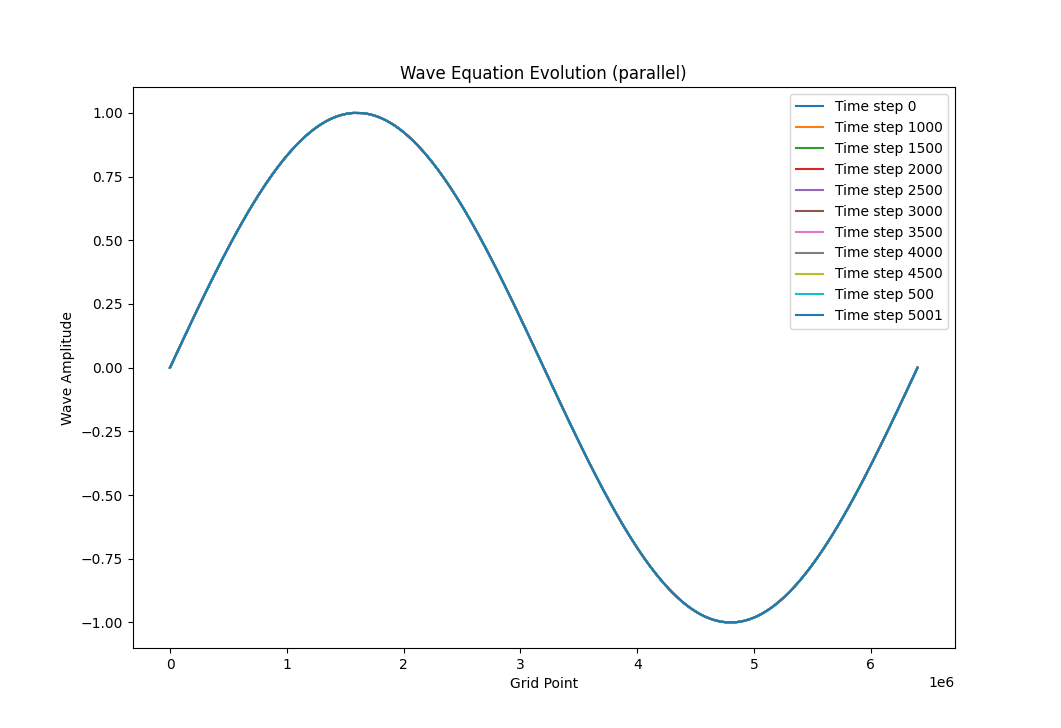
\includegraphics[width=\linewidth]{img/ex1/wave_vis_parallel.png}
        \caption{Parallel Output}
        \label{fig:ex1_parallel_output}
     \end{subfigure}
     \hfill
     \begin{subfigure}[b]{0.45\textwidth}
        \centering
        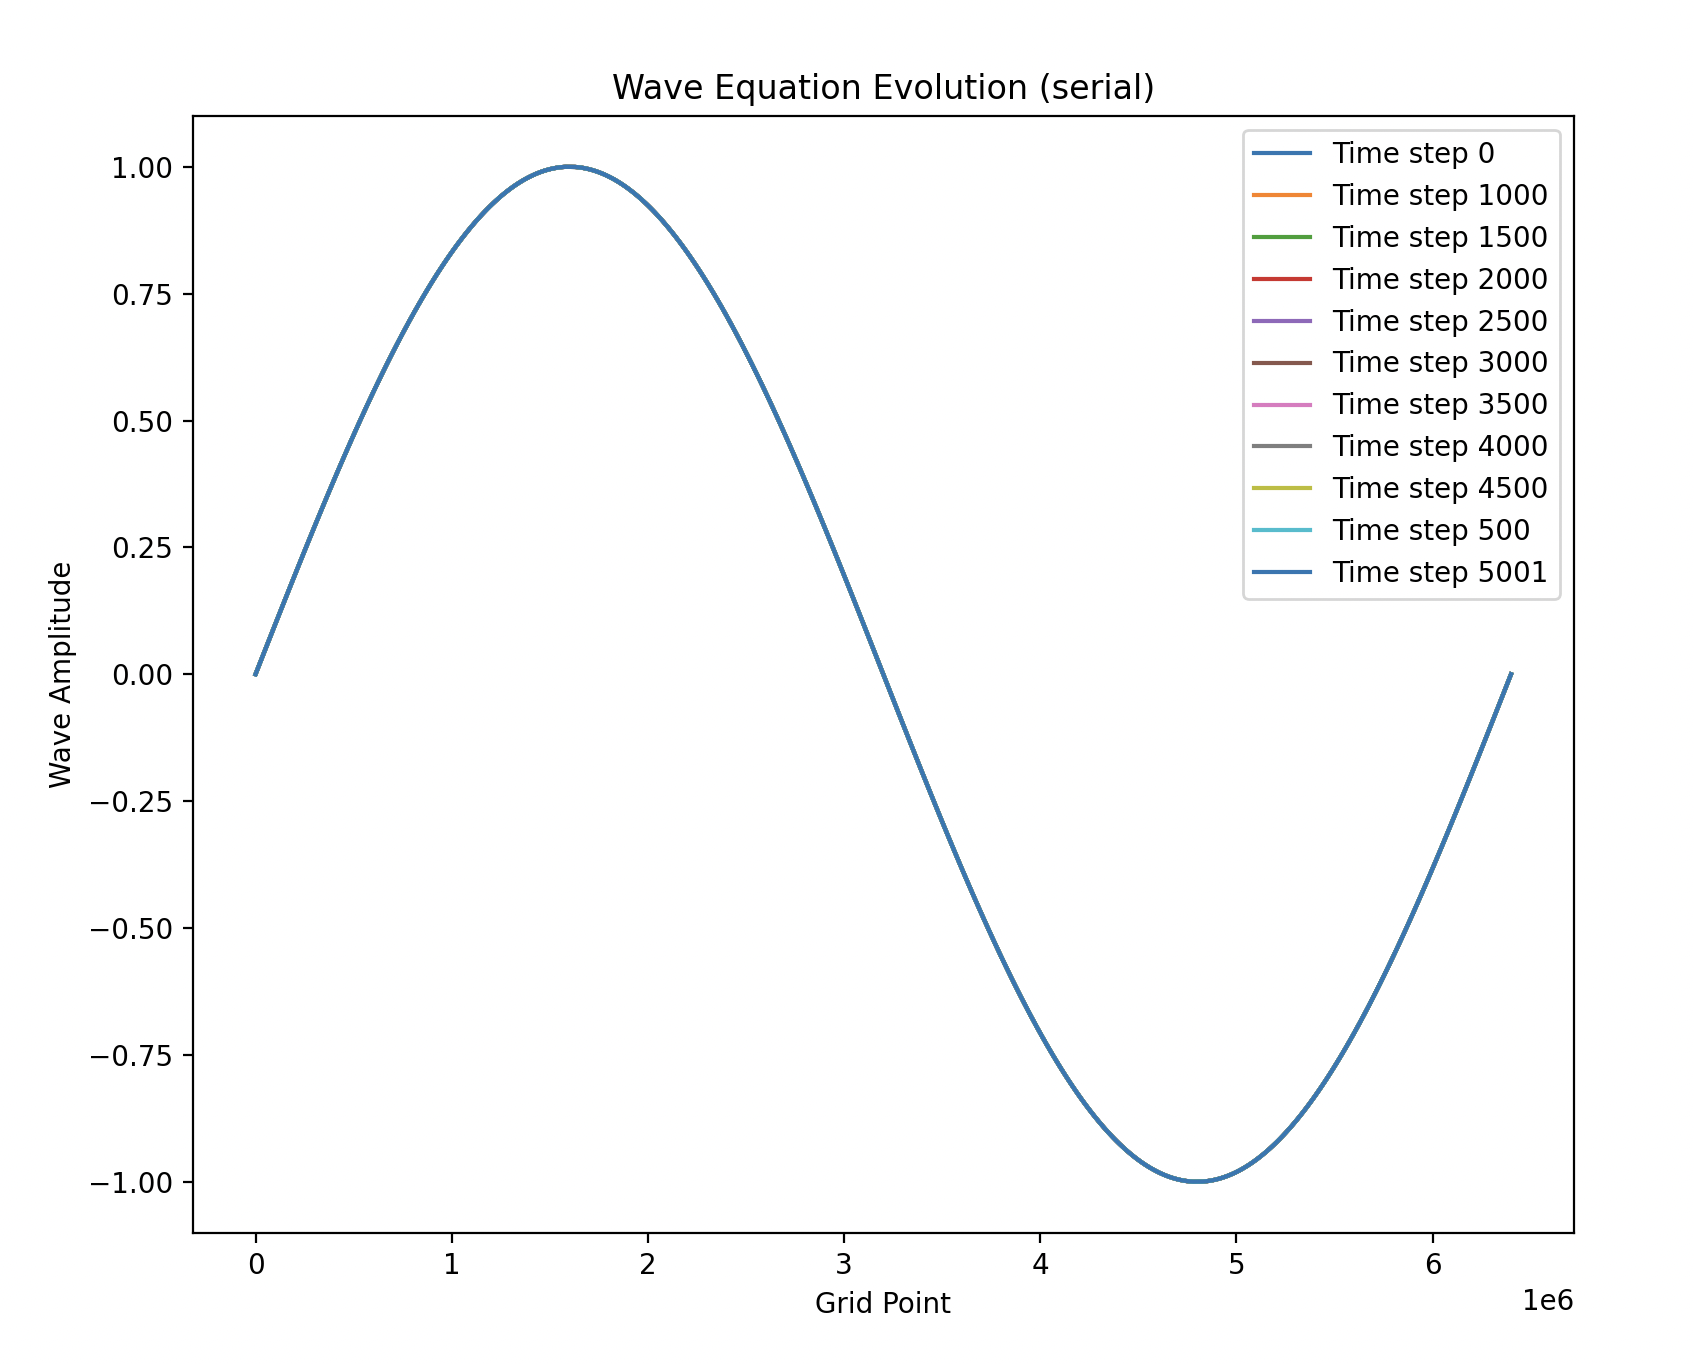
\includegraphics[width=\linewidth]{img/ex1/wave_vis_serial.png}
        \caption{Serial Output}
        \label{fig:ex1_serial_output}
     \end{subfigure}
  \caption{Parallel and Serial Outputs}
\end{figure}

To generate this plot, the following command can be run form under the \verb|ex1/| directory: 

\begin{center}
\verb|python3 visualize.py --mode {parallel/serial}|
\end{center}

To further ensure that the outputs were identical, a bash script was created: \verb|verify_outputs.sh|. This individually checks for diffs between the parallel and the serial implmenetation output, failing if the parallel and serial files for any timestamp are not identical. It can be found \href{https://github.com/paulmyr/DD2356-MethodsHPC/blob/master/4_mpi/ex1/verify_outputs.sh}{here} and is run using \verb|sh verify_outputs.sh| from under the \verb|ex1/| directory. 

\subsection{Runtime Analysis}
For this analysis, we used $N = 6.4\text{ million}$ and $STEPS = 5000$. The plots were generated with the python file \verb|plotting.py| in the \verb|ex1/| directory. The runtimes plotted below were obtained from the results in the \verb|outputs/runtimes| directory. 

\subsubsection{Runtime for Different Process Counts}
\label{sec:diff_process_counts}
The runtime for different number of processes compared to the serial implementation can be seen in Figure \ref{fig:ex1_process_counts}. For this, we used the configuration in the \verb|run_sim_vary_process.sh| file (found \href{https://github.com/paulmyr/DD2356-MethodsHPC/blob/master/4_mpi/ex1/run_sim_vary_process.sh}{here}), where we allocated 1 node with 64 tasks per node and 1 cpu per task.

\begin{figure}[H]
  \centering
  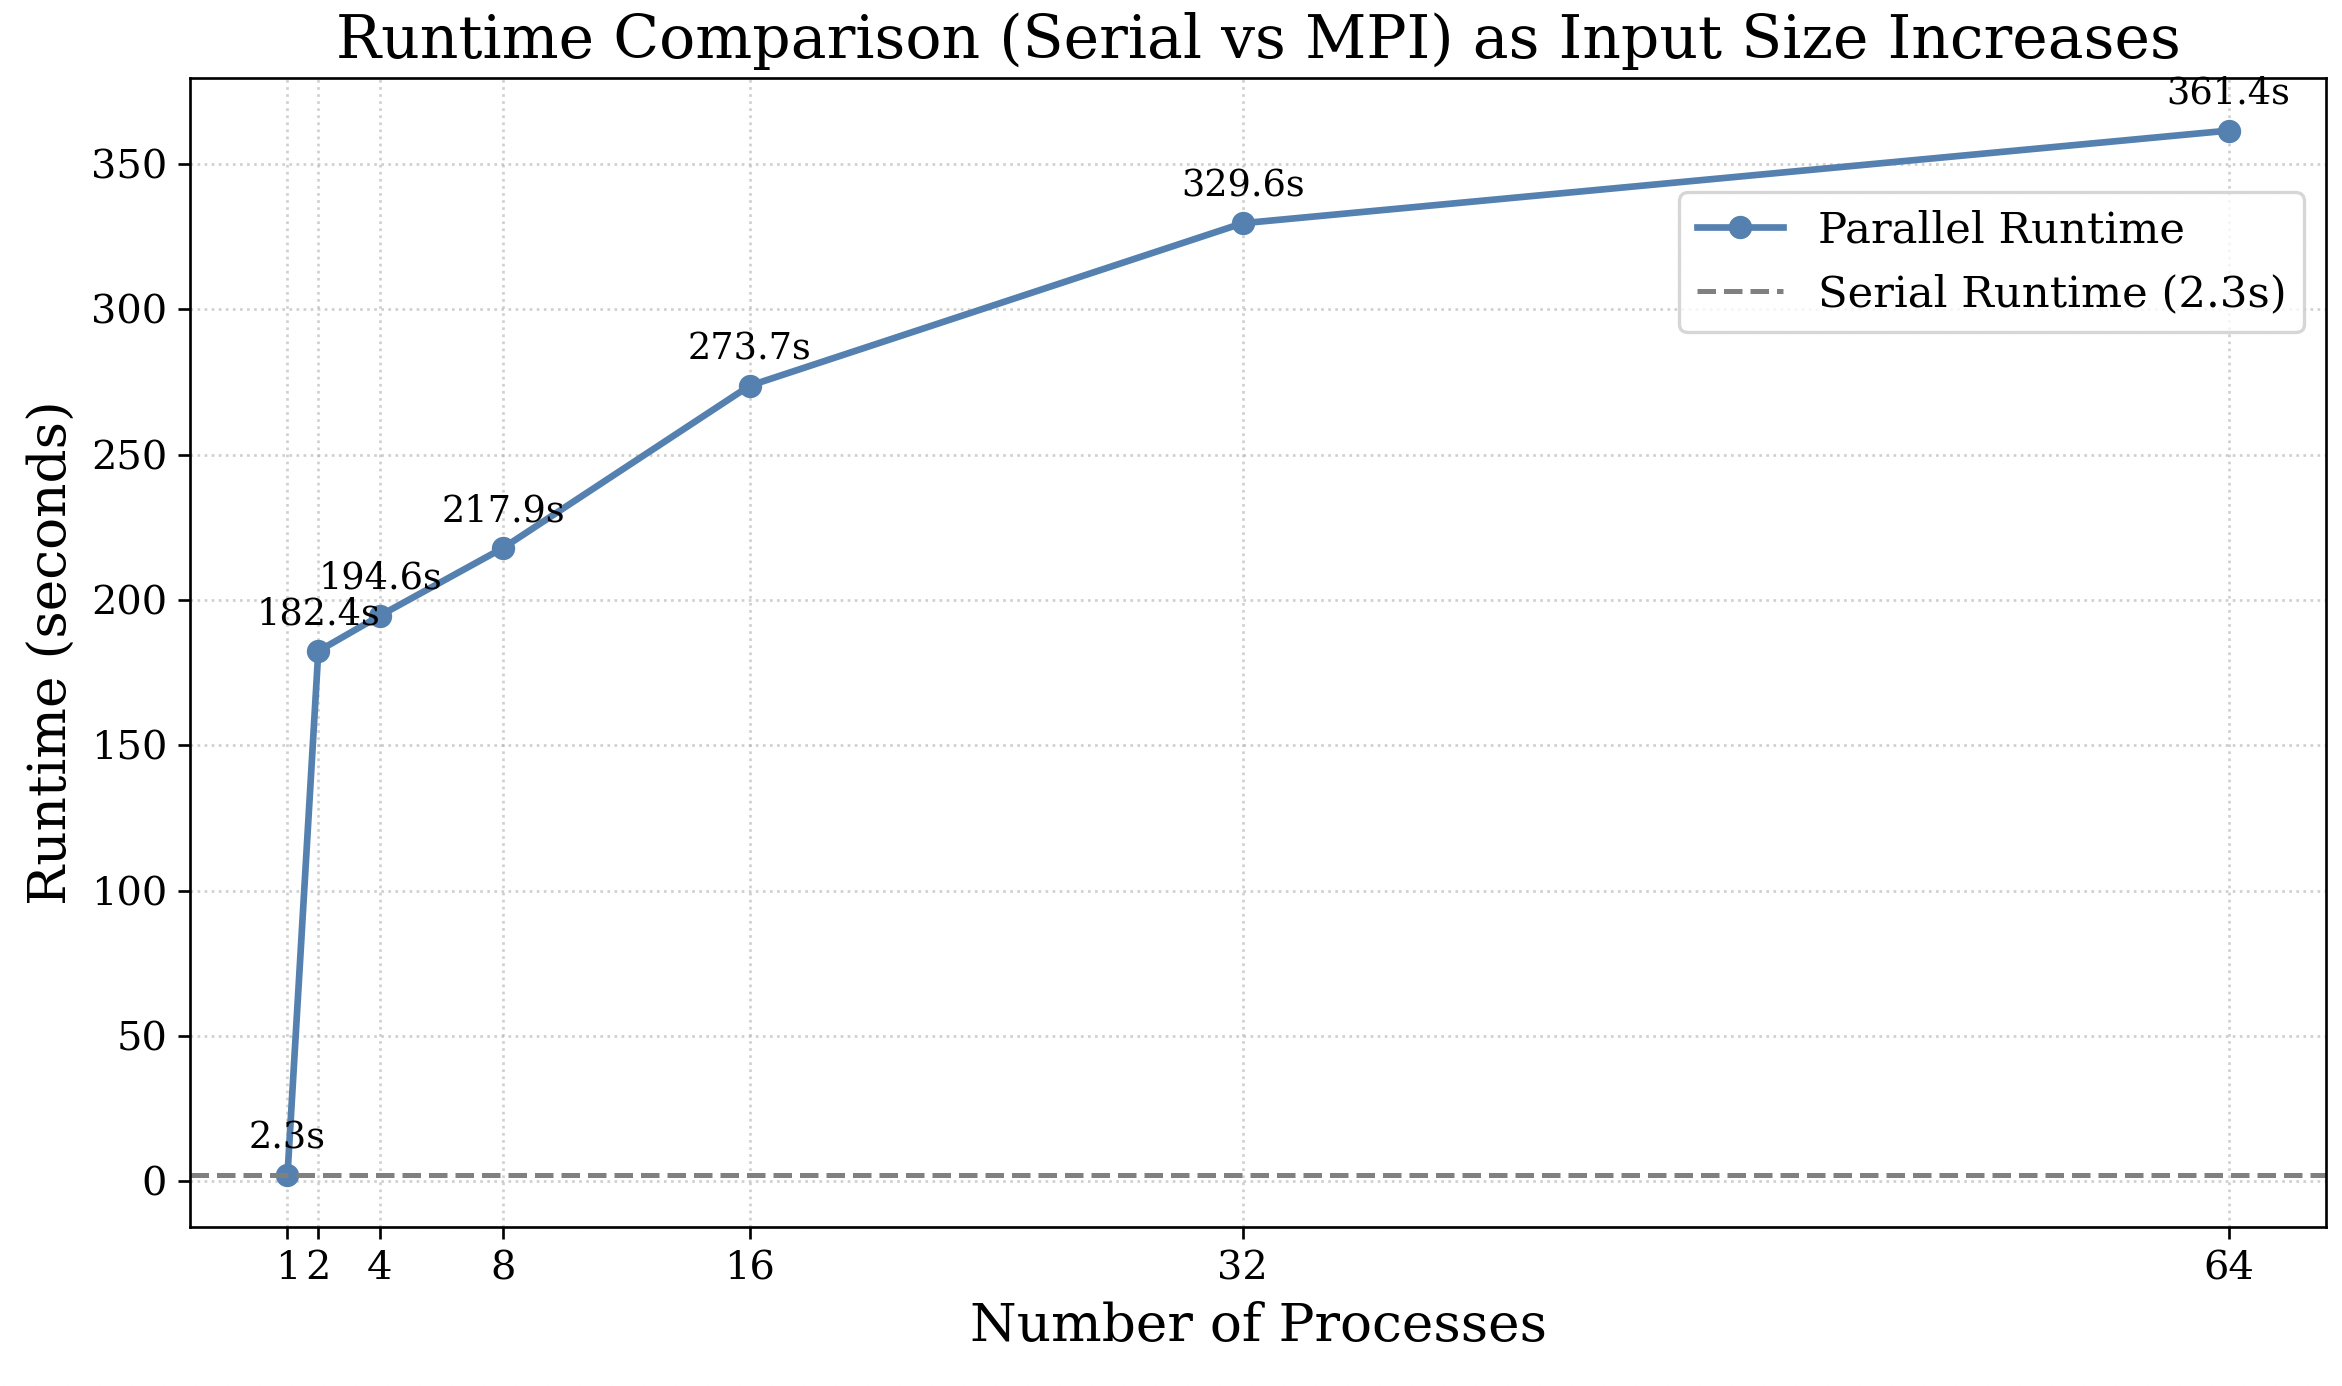
\includegraphics[width=0.9\textwidth]{img/ex1/serial_vs_mpi}
  \caption{Serial vs MPI Comparison for Different Process Counts}
  \label{fig:ex1_process_counts}
\end{figure}
As can be seen from the figure, after a worse runtime for 1 and 2 processes, the runtime for higher number of processes is lower compared to the serial runtime. We believe that the high runtime for 1 or 2 processes could be attributed to the fact that there is greater MPI related overhead compared to the benefits achieved from the limited parallelism offered by 1 or 2 processes.
 
However, as the number of processes increase and the amount of work that needs to be done remains the same, we start to see the benefit of this work being done in parallel by multiple processes. The lowest runtime achieved seems to be from 16 processes, indicating that after this, the benfit of parallelism diminishes likely because of the greater MPI overhead (exchanging ghost cells between more processes, barrier at the end of computation waiting for more processes, etc). However, even after the slight increase, the runtime at 64 processes is considerably less than the serial, which shows the clear benefit of parallelism through MPI. 

\subsubsection{Runtime for Different Node Counts}
When chaning the number of nodes, we kept all other elements ($N$, $STEPS$, processes, etc) constant. We measured with a total of 32 processes, distributed equally amongst 1, 2, 4, 8, and 16 nodes. This means that when operating with 2 nodes, each node had 16 processes, when using 4 nodes, each node had 8 processes, and so on. For each node count (except for 1 node, where we already had the runtime from above), the respective job-file is titled \verb|run_sim_nodes_<count>.sh| in the code. 

Given this setup, the runtime across different nodes compared to the serial implementation can be seen in Figure \ref{fig:ex1_node_counts}.
\begin{figure}[H]
  \centering
  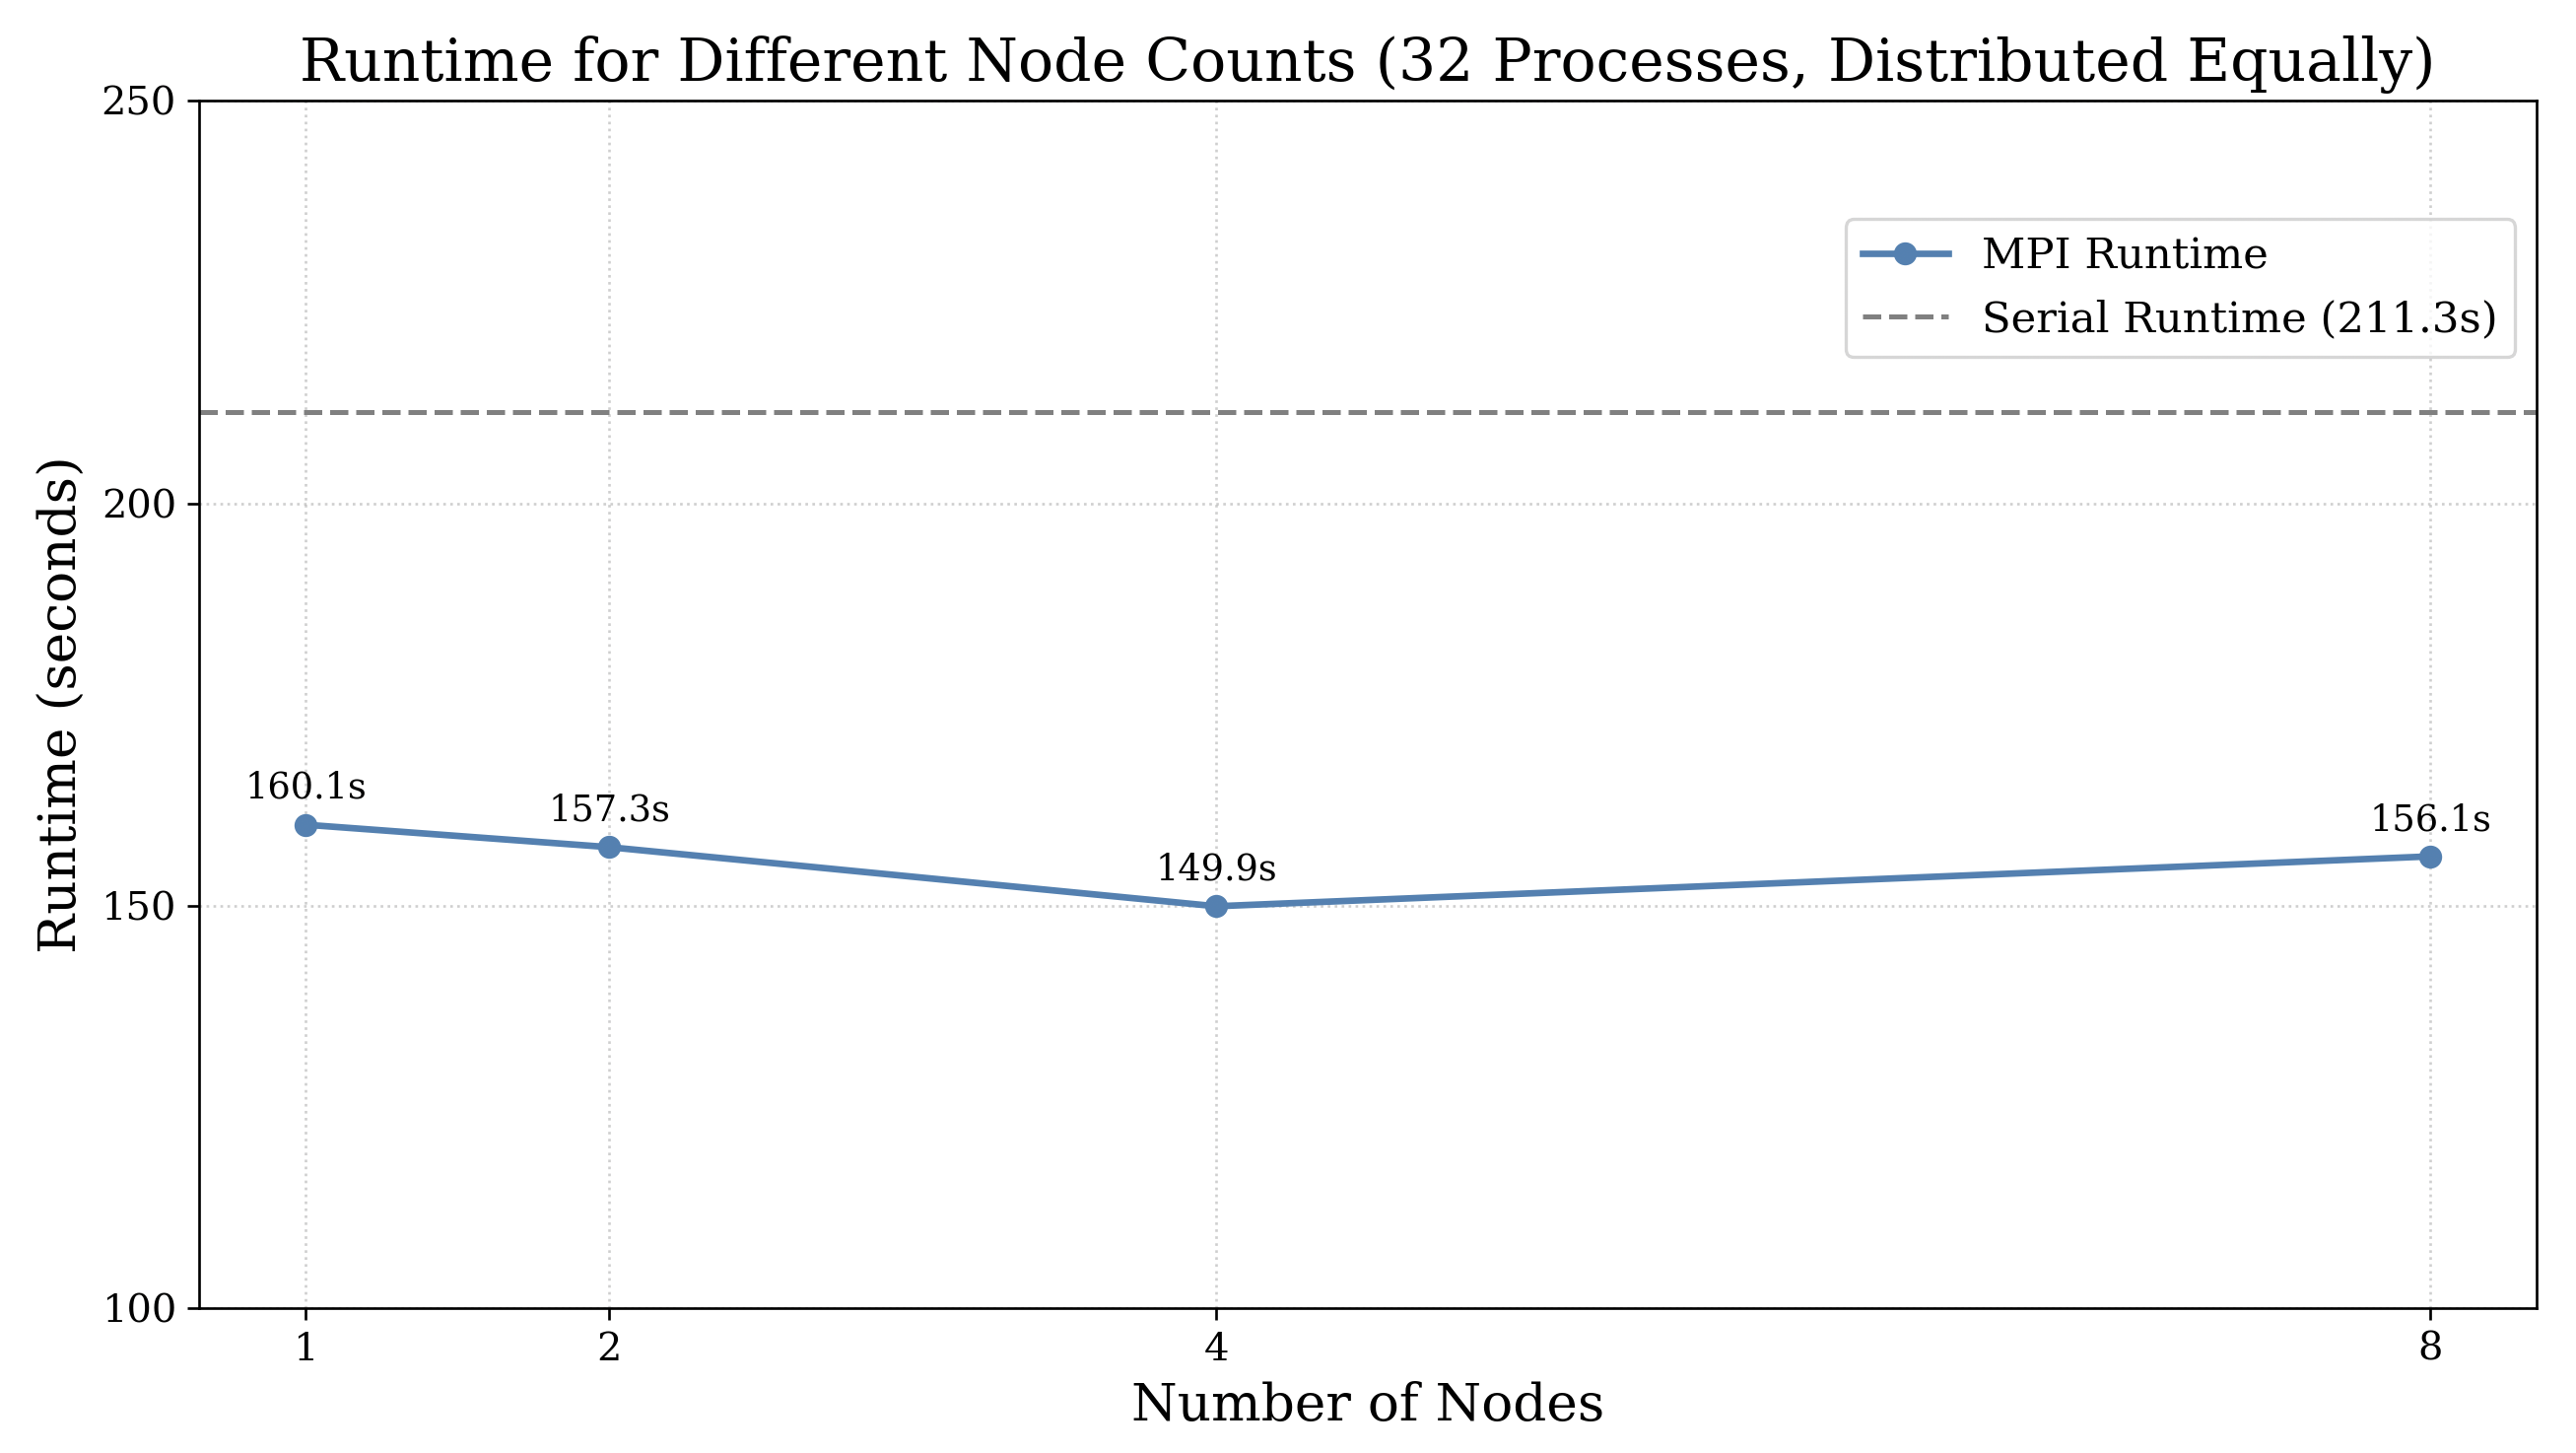
\includegraphics[width=0.9\textwidth]{img/ex1/diff_node_counts}
  \caption{Serial vs MPI Comparison for Different Process Counts}
  \label{fig:ex1_node_counts}
\end{figure}

As can be seen from the figure, the runtime across different node counts is considerably lower than the serial runtime on 1 node. This indicates that despite the possible network-overhead involved with communication over different nodes, the benefits of MPI parallelism compared to the serial version far outweigh the potential downsides. The lowest runtime seems to be across 2 nodes, and increases slightly as the number of nodes increase. This seems to be in-line with our expectations: distributing across 2 nodes might help in reducing the load on a single node while keeping inter-node network communication within a reasonable limit -- giving better runtimes. However, as the number of nodes increase, so does the inter-network communication overhead, which slightly decreases the efficiency. 

However, we'd note that the trend doesn't seem to be as large as we had expected. To us, this might indicate that inter-network node communication might not be the leading factor contributing to the runtime of the MPI implementation. The blocking nature of \verb|Sendrecv|, which prevents us from overlapping computation with communication, and other optimizations can further be applied to improve the runtime even more across several nodes. 

\subsubsection{Strong and Weak Scaling}
The Strong-Scaling Test -- keeping the overall problem size constant while increasing the number of processes -- was already performed when varying the process counts. We present the graph again in Figure \ref{fig:ex1_strong_scaling} but refrain from repeating our analysis which can be found in Section \ref{sec:diff_process_counts}. 
\begin{figure}[H]
  \centering
  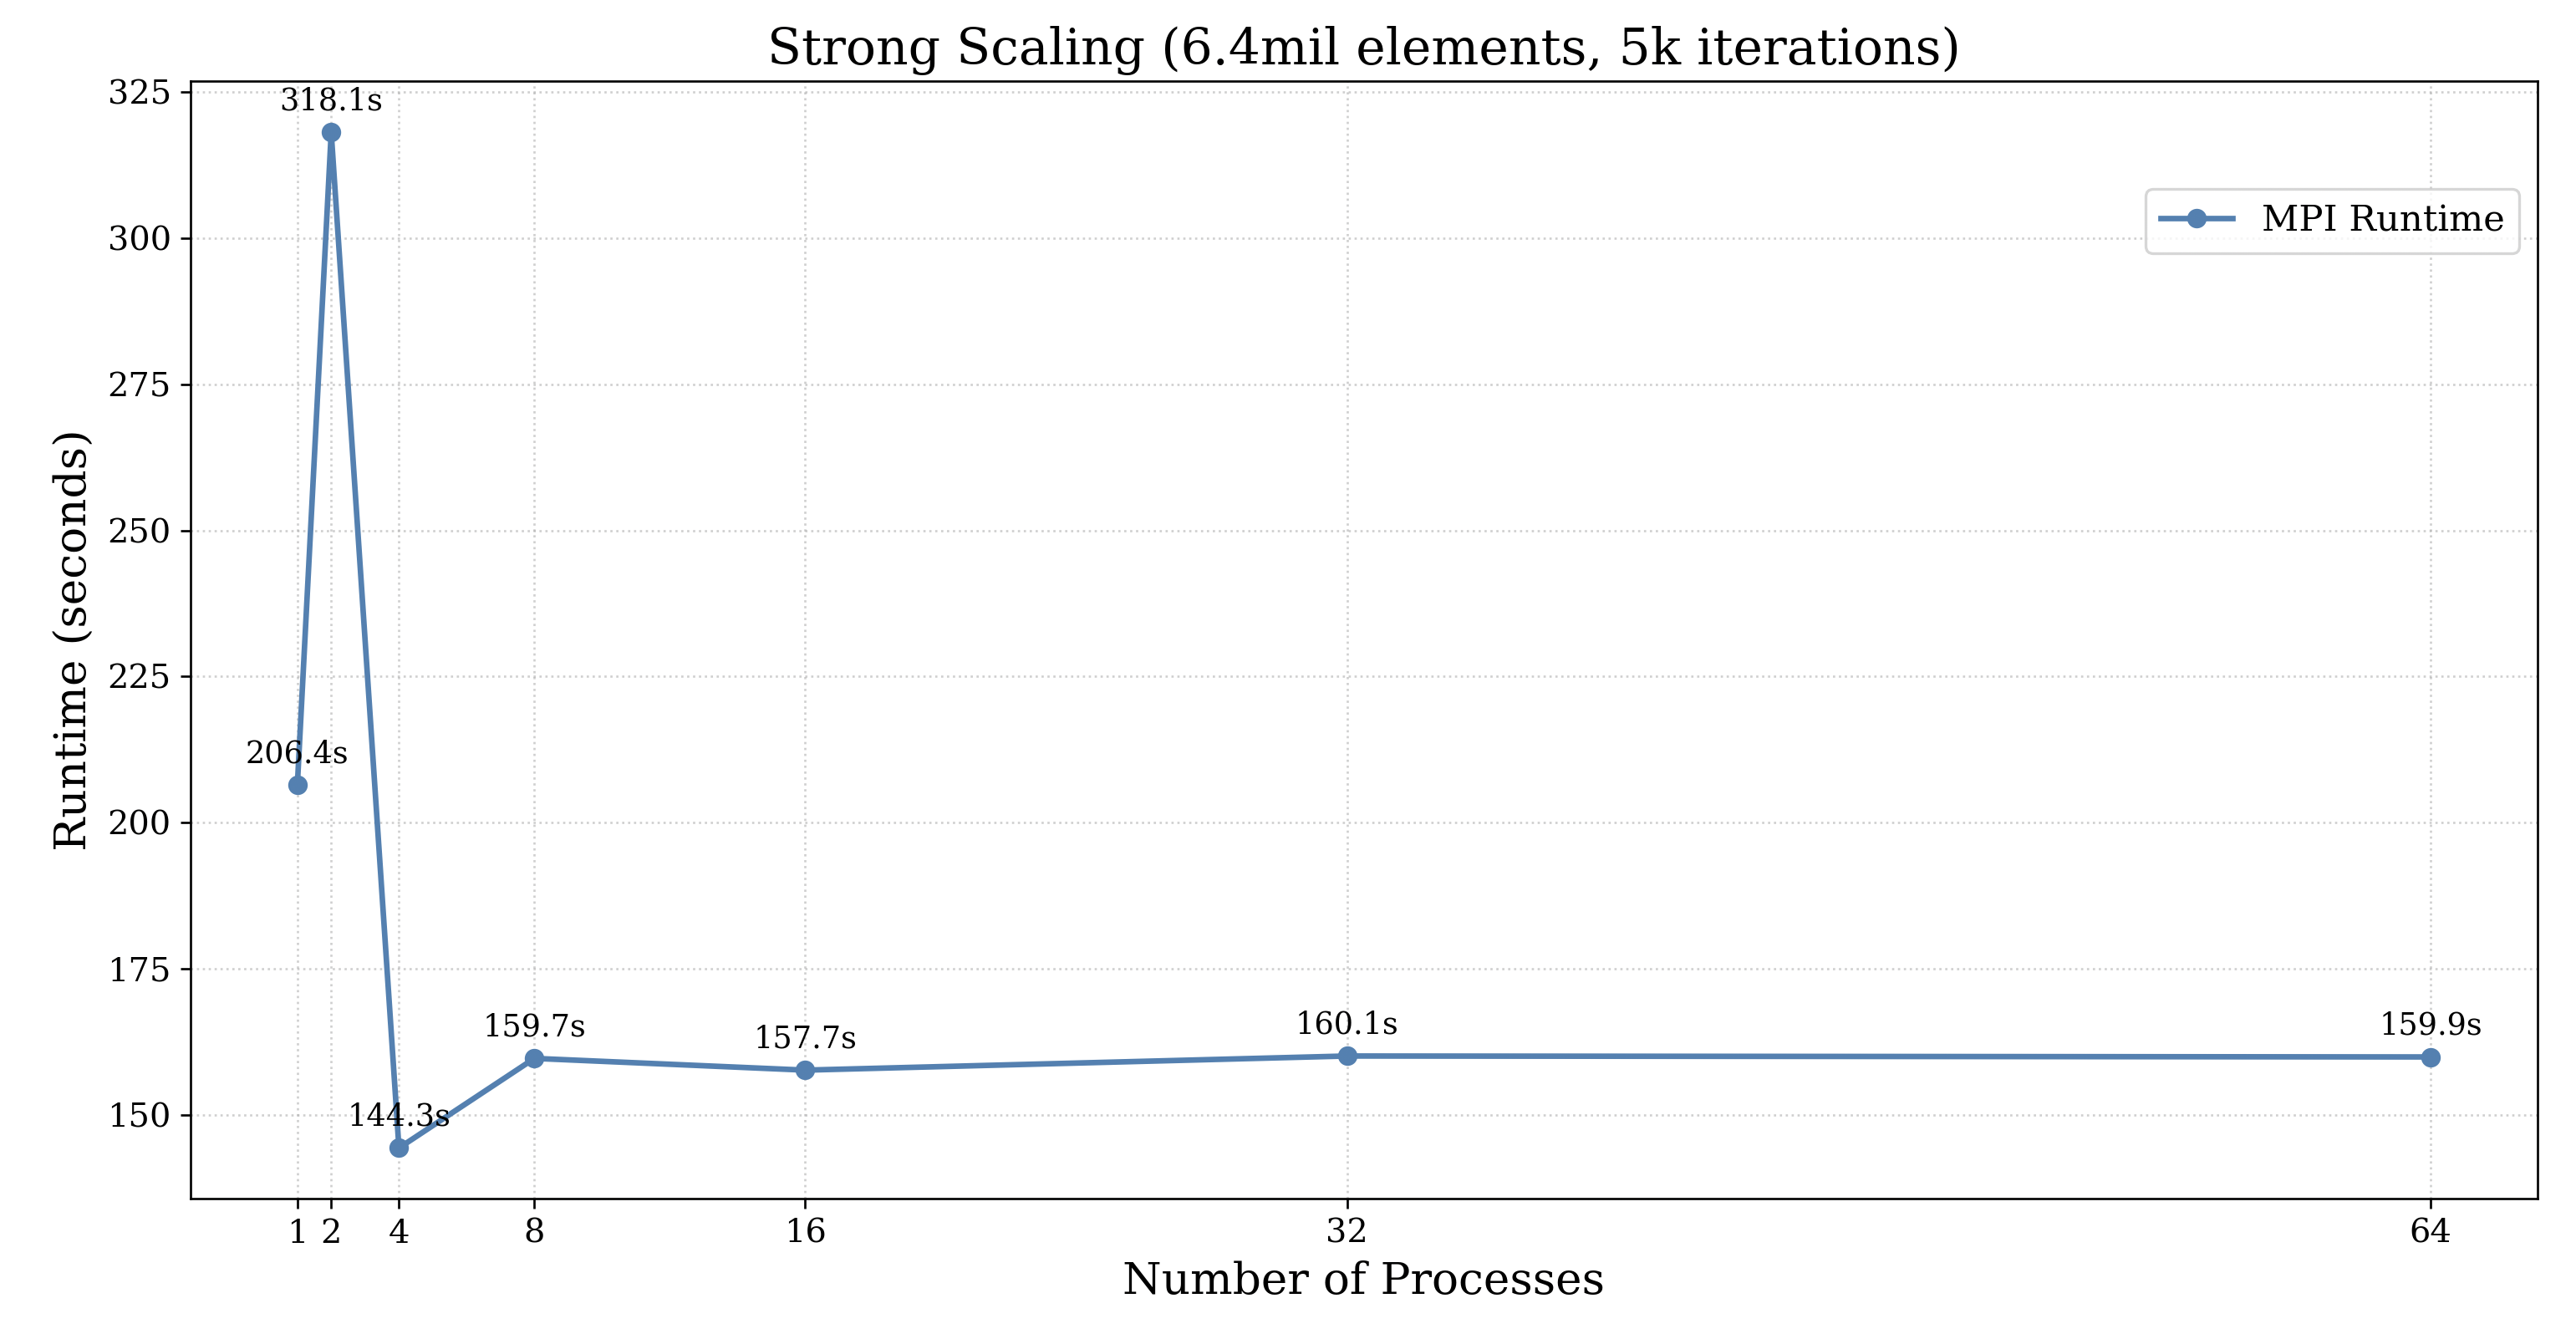
\includegraphics[width=0.9\textwidth]{img/ex1/strong_scaling}
  \caption{Strong Scaling}
  \label{fig:ex1_strong_scaling}
\end{figure}

The Weak-Scaling Test -- where the problem size per process is the same as the number of processes increase -- was performed by fixing 100k elements of the global array per process and 5k iterations. The job-script for this test was \verb|run_sim_weak_scaling.sh|. Figure \ref{fig:ex1_weak_scaling} presents the runtime output. 
\begin{figure}[H]
  \centering
  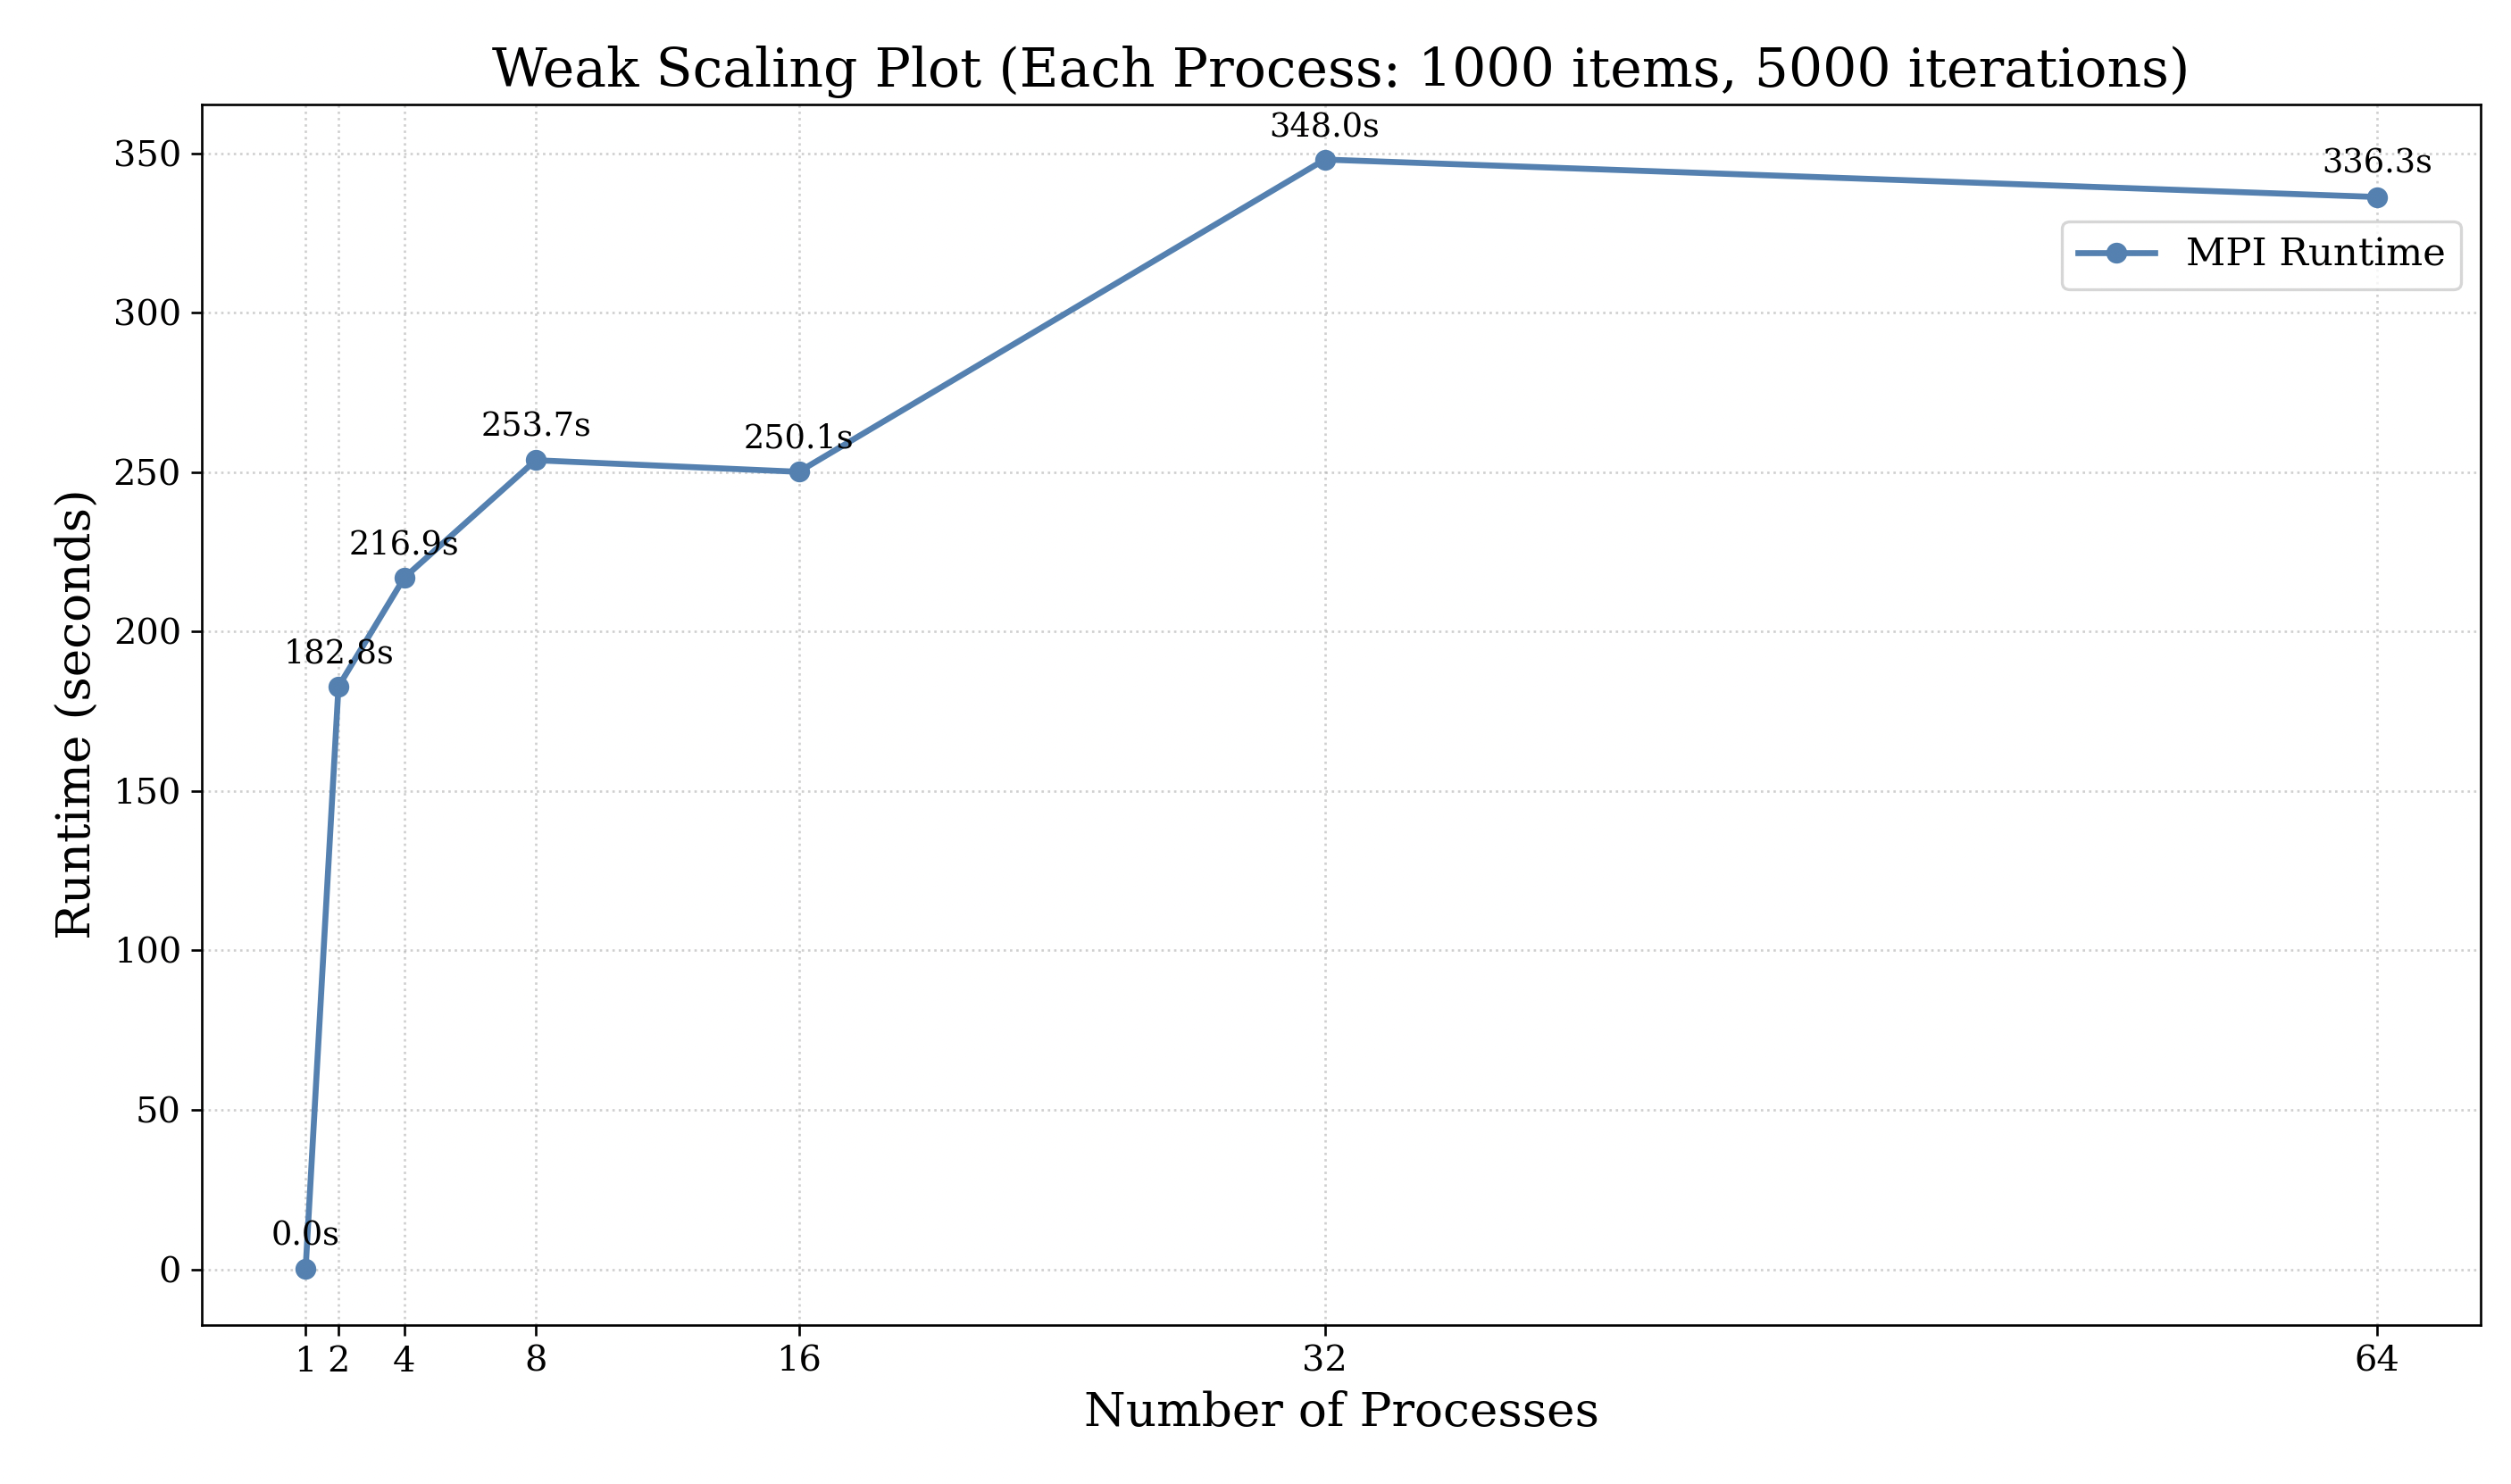
\includegraphics[width=0.9\textwidth]{img/ex1/weak_scaling}
  \caption{Weak Scaling}
  \label{fig:ex1_weak_scaling}
\end{figure}
The ideal scenario of a weak-scaling test to us would be similar runtimes as the number of processes (and thus the problem size) increases. This is because such a behaviour would indicate that larger problem sizes can be efficiently solved by increasing the number of resources (processes in our case) available to tackle them. Based on our understanding, the results we obtain largely adhere to the this ideal scenario.

We see a sharp increase in the runtime on going from 1 process to 2 processes. This is within our expectations: as there is now communication and syncronization overhead involved with multiple processes in the picture. There is a noticeable decrease in the runtime on going from 4 to 8 processes, which to us is an excellent obseration -- as this would indicate that the implementation is scaling well: larger problem sizes can be solved even more quickly with larger processes available. The runtime then begins to increase slightly, reaching the range of 150s again as we go to 64 processes. 

However, in all cases (except for the case with 1 sole process, the reasoning for which we gave above), the runtime remains similar as the problem size increases with the number of processes -- which was our expected ideal behaviour. At times, it seems to even perform better: decreasing with an increase in the number of processes and the problem size (like with 8 processes). 

\section{Parallel Row Sum Computation using MPI Collectives}
We started by running the code in the seqential version:
The generated image looks as follows:
\begin{figure}[H]
  \centering
  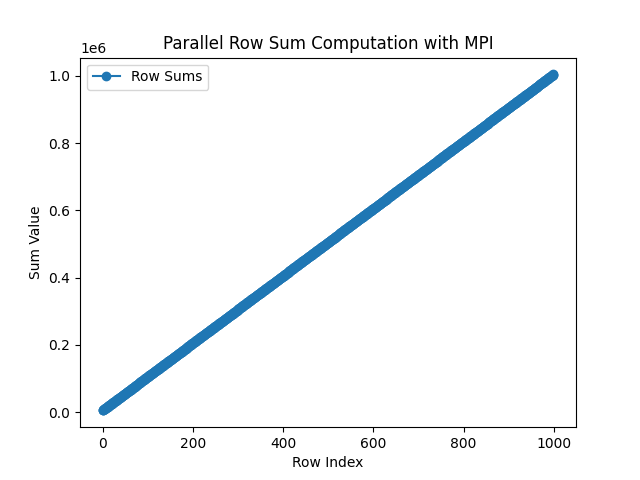
\includegraphics[width=0.9\textwidth]{img/ex2_seq}
  \caption{row summation using sequential implementation.}
  \label{fig:ex2_seq}
\end{figure}

To paralleise the code, we use \verb|MPI_Scatter(...)|.
To use MPI, we first initialise the application.

\lstinputlisting[language=C, firstline=62, lastline=66]{ex2/parallel_row_sum.c}

The main idea, is to distribute the matrix equally onto the available threads.
Our strategy is to split the matrix into chunks, each chunk contains an equal number of rows.
To achieve this, we first compute the chunk size, which is the number of rows each thread has to compute.
The basic formula for this is $\frac{N}{M}$, where $N$ is the number of rows and $M$ is the number of threads.
Because by default $N$ does not have to be divisible by $M$, we pad the matrix so that it has length $N^*$, where $N^* \mod M = 0$.
\lstinputlisting[language=C, firstline=75, lastline=77]{ex2/parallel_row_sum.c}
We initialize the matrix only on the root process and use scatter to distribute it to the rest of the threads.
This can be achieved by the following code:
\lstinputlisting[language=c, firstline=79, lastline=93]{ex2/parallel_row_sum.c}
Note, that the full matrix is only allocated on the root process!
The summation is then done on subsets of the matrix individually.
We gather all the solutions by using \verb|MPI_Gather(...)|:
\lstinputlisting[language=c, firstline=97, lastline=108]{ex2/parallel_row_sum.c}

The image looks identical to the sequential version:
\begin{figure}[H]
  \centering
  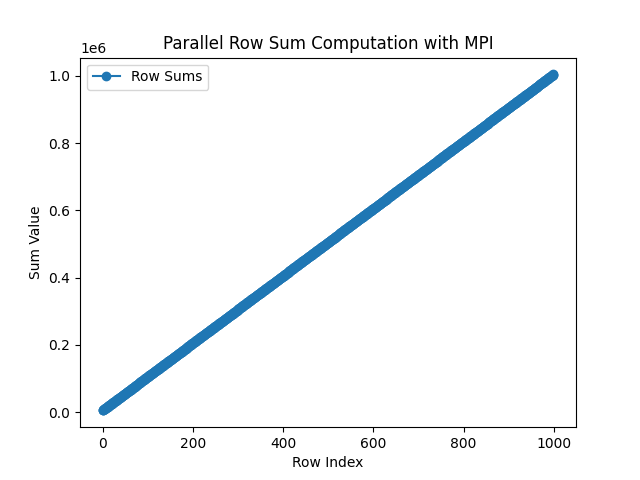
\includegraphics[width=0.9\textwidth]{img/ex2_para}
  \caption{row summation using parallel implementation.}
  \label{fig:ex2_seq}
\end{figure}

To compute the total sum, we first reduce the local result into a single local sum.
These we can then reduce globally using \verb|MPI_Reduce(...)|:
\lstinputlisting[language=c, firstline=110, lastline=113]{ex2/parallel_row_sum.c}
Note that for large matrices (depending on initialisation) this will lead to overflows!

\todo[inline]{ex2 scaling tests...}

\section{Profiling MPI applications with Score-P and Vampir}

\section{HPC Libraries -Matrix-Vector Multiplication using BLAS}

\section{Bonus: 2D Game of Life with MPI and Non-Blocking Communication}

% content end
%###############################################################################

% \printbibliography

\end{document}
